\section{Bitmap}

\subsection{Pourquoi le bitmap?}
Le format BITMAP aussi appelé DIB (Device Independent Bitmap) a été conçu par Windows corporation pour pouvoir échanger des images entre devices sans avoir à se soucier de la logique de ceux-ci.
Ces images ont des extensions .bmp ou encore .dib.
Techniquement, une image bitmap est un format de fichier non compressé, cela signifie entre autre que chaque pixel possède sa représentation sous forme d'un bit ou d'une série de bits.
On peut donc opposer sa structure à celle d'une image PNG, JPEG ou encore GIF qui utilise la compression pour regrouper des pixels similaires afin de réduire la taille globale du fichier.
On les appelle donc bitmaps car ils ne sont pas compressés (possible de le faire cependant).
Ils n'ont donc aucune perte de données et sont donc par conséquent, bien plus grandes.\\

La structure du format BITMAP est connue et disponible en ligne. En voici un schéma : \\\\

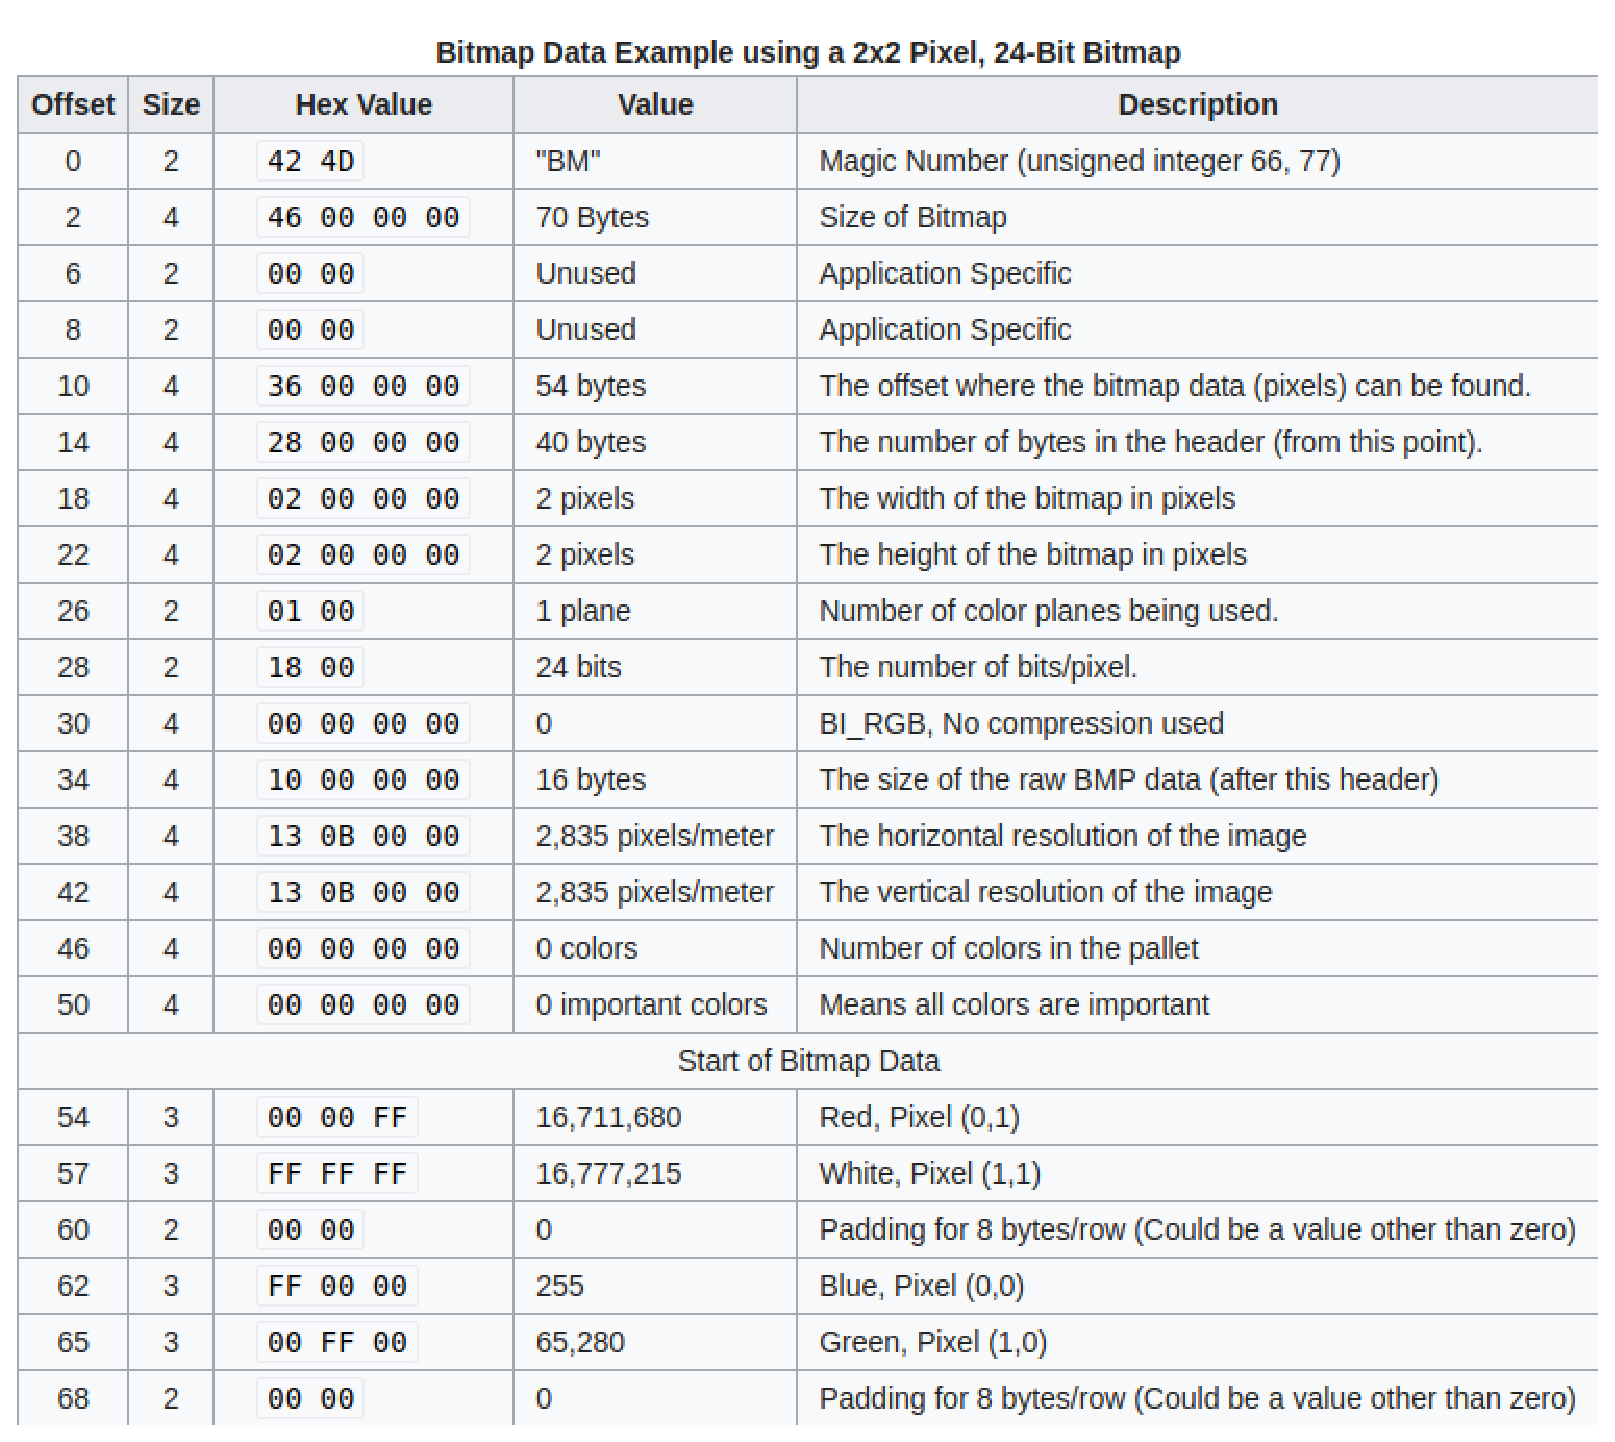
\includegraphics[width=15cm]{bitmap_structure.eps}\\\\

\subsection{Application du LSB}
Nous avons choisi de cacher des informations à partir du 11ème byte du header. 
Cela nous permet d'amoindrir les altérations de l'image en sortie.
Notre premier choix était de modifier les bits de pixels de l'image donc à partir du 54ème byte mais l'image semblait fortement modifiée.

\subsection{Avancement}
Dans un premier temps, les pixels de l'image sont considérés comme étant une suite de 8 bits par pixel sans tenir compte du fait que le nombre de bits par pixel peut varier.
Cela offre une réflexion supplémentaire qui permettrait d'expliquer pourquoi avec notre approche, on ne peut pas uniquement cibler la zone des pixels de l'image sans altérer complètement celle-ci.
Il nous faudra dans une prochaine remise travailler à améliorer cet aspect et ainsi tenir compte de ces paramètres.
